%-----------------------------------------------------------------%
% 2015 - 2025 Emerson Ribeiro de Mello - mello@ifsc.edu.br
% 
% 2025/04/16 versão 2
% 
% Modelo de monografia para o Instituto Federal de Santa Catarina
% 
% Adaptação do documento abnTeX2: Modelo de Trabalho Acadêmico
% para ficar de acordo com o "Manual de normalização de trabalhos
% acadêmicos do Sistema de Bibliotecas integradas do IFSC (SiBI/IFSC)  - rev 08abr25"
% disponível em  https://www.ifsc.edu.br/documentos-uteis. Acessado em 2025-04-16
%-----------------------------------------------------------------%
\documentclass[
    12pt,				% tamanho da fonte
    openright,			% capítulos começam em pág ímpar (insere página vazia caso preciso)
    oneside,			% para impressão em frente e verso, use "twoside"
    a4paper,			% tamanho do papel. 
    % -- opções da classe abntex2 --
    chapter=TITLE,		% títulos de capítulos convertidos em letras maiúsculas
    section=TITLE,		% títulos de seções convertidos em letras maiúsculas
    english,			% idioma adicional para hifenização
    brazil				% o último idioma é o principal do documento
]{ifscthesis}

% Para gerar texto de exemplo
\usepackage{lipsum} 

% Arquivo com as referências bibliográficas
\addbibresource{referencias.bib}


% Capa

%-----------------------------------------------%
% Para alterar o gênero dos comandos orientador
% e coorientador.
%-----------------------------------------------%
% \renewcommand{\orientadorname}{Orientadora:}
\renewcommand{\coorientadorname}{Coorientadora:}
%-----------------------------------------------%


%-----------------------------------------------%
% Informações de dados para CAPA e FOLHA DE ROSTO
%-----------------------------------------------%
\titulo{Estudo e Implementação dos Algoritmos de Compressão LZ77 e Codificação
Aritmética na Biblioteca Komm}
\autor{Rhenzo Hideki Silva Kajikawa}

\local{São José}
\data{2025}

\orientador{ Prof. Roberto Wanderley da
Nóbrega, Dr.}

\instituicao{%
  INSTITUTO FEDERAL DE EDUCAÇÃO, CIÊNCIA E TECNOLOGIA DE SANTA CATARINA
  \par
  CAMPUS SÃO JOSÉ
  % \par
  % ÁREA DE TELECOMUNICAÇÕES
}

  \tipotrabalho{Monografia (Graduação)

}



% O preambulo deve conter o tipo do trabalho, o objetivo, o nome da instituição e a área de concentração 
\preambulo{Monografia apresentada ao Curso de Engenharia de Telecomunicações do Instituto Federal de Santa Catarina, para a obtenção do título de bacharel em Engenharia de Telecomunicações.

\vspace*{.3cm}

Área de concentração: Telecomunicações
}




% Abreviaturas, siglas e símbolos
\makeglossaries
% \setabbreviationstyle[acronym]{long-postshort-user}
\setabbreviationstyle[acronym]{long-short-user}
\glssetcategoryattribute{acronym}{nohyperfirst}{true}
% \glssetcategoryattribute{acronym}{nohyper}{true}

% ------------------------------------%
%  Como usar os comandos do glossário
% ------------------------------------%
% \gls{TLS} - Na 1a. vez, texto por extenso + sigla. Nas chamadas subsequentes somente a sigla
% \glspl{IdP} - Para colocar s como prefixo da sigla
% \Gls{} - Inicial em maiúscula
% \glsxtrfull{} - texto por extenso + sigla
% \glsxtrfullpl{} - texto por extenso no plural + sigla
% \glsxtrshort{} - somente a sigla
% \glsxtrlong{} - somente o texto por extenso

%  Caso queira criar uma entrada que tenha tradução para inglês, use o parâmetro user1. 
%      Veja exemplo abaixo para Credenciais Verificáveis
% 
% Caso queira criar plural, use o parâmetro longplural. Veja exemplo para IAA
% ------------------------------------%

\newacronym
{json} % rótulo 
{JSON} % sigla
{\textit{JavaScript Object Notation}} % por extenso


\newacronym{ABNT}{ABNT}{Associação Brasileira de Normas Técnicas}

\newacronym{abnTeX}{abnTeX}{ABsurdas Normas para TeX}

\newacronym[longplural={Autoridades Certificadoras}]{AC}{AC}{Autoridade Certificadora}

\newacronym{AES}{AES}{\textit{Advanced Encryption Standard}}

\newacronym{TLS}{TLS}{\textit{Transport Layer Security}}

\newacronym{TPC}{TPC}{Terceira Parte Confiável}

\newacronym{IFSC}{IFSC}{Instituto Federal de Santa Catarina}
\glsxtrnewsymbol[description={conjunto vazio}]
{emptyset}% rótulo (será usado na ordenação na lista de símbolos)
{\ensuremath{\emptyset}}% símbolo


\glsxtrnewsymbol[description={número Pi}]
{pi}% rótulo (será usado na ordenação na lista de símbolos)
{\ensuremath{\pi}}% símbolo


\begin{document}
% Seleciona o idioma do documento (conforme pacotes do babel)
\selectlanguage{brazil}




%-----------------------------------------------%
% ELEMENTOS PRÉ-TEXTUAIS
%-----------------------------------------------%
\imprimircapa
\imprimirfolhaderosto

%-----------------------------------------------%
% Ficha catalográfica
%-----------------------------------------------%

% Pegue com a Biblioteca do IFSC um PDF com a 
% ficha correta, salve o arquivo no diretório
% deste projeto e descomente as linhas abaixo

% \begin{fichacatalografica}
%     \includepdf{ficha-catalografica.pdf}
% \end{fichacatalografica}

%-----------------------------------------------%
% folha de aprovação
%-----------------------------------------------%
\begin{folhadeaprovacao}

    \begin{center}
        {\ABNTEXchapterfont\normalfont\large\imprimirautor}

        \vspace*{2cm}

        \ABNTEXchapterfont\normalfont\large\imprimirtitulo
        
    
        \vspace*{2cm}

\hspace{.45\textwidth}
\begin{minipage}{.5\textwidth}
\SingleSpacing
{\normalsize Monografia apresentada ao Curso de Engenharia de Telecomunicações do Instituto Federal de Santa Catarina, para a obtenção do título de bacharel em Engenharia de Telecomunicações.}
\end{minipage}%
        
        \vspace*{2cm}

        % Essa data de aprovação deve ser colocada após a defesa e aprovação do trabalho
        \imprimirlocal, 16 de abril de 2025.

    \end{center}

    \vfill

    \setlength{\ABNTEXsignskip}{1.5cm}
    \assinatura{\imprimirorientador \\[.5em] Instituto Federal de Santa Catarina}     
    \assinatura{Professor Fulano, Dr. \\[.5em] Instituto Federal de Santa Catarina }
    \assinatura{Professora Fulana, Dra.  \\[.5em] Instituto Federal de Santa Catarina}
    % \assinatura{\textbf{Professor Beltrano, Dr.} \\[.5em] Instituto Z}
  
\end{folhadeaprovacao}
%-----------------------------------------------%

\begin{dedicatoria}
\vspace*{\fill}
\begin{flushright}
\begin{minipage}{0.5\textwidth}
        
    Aos meus pais, que sempre acreditaram em mim, e me ensinaram a sonhar.

\end{minipage}
\end{flushright}
\vspace*{3cm}
\end{dedicatoria}
\begin{agradecimentos}
    
    Agradeço à minha família, que sempre esteve ao meu lado, me apoiando e incentivando a seguir em frente. Vocês são a minha base e a razão pela qual busco sempre o melhor.
    
    Agradeço especialmente ao meu orientador, Professor Fulano, pela orientação e apoio durante todo o processo de elaboração deste trabalho. Sua experiência e conhecimento foram fundamentais para o meu aprendizado e crescimento acadêmico.
    
    Agradeço ao Instituto Federal de Santa Catarina, que me proporcionou uma formação sólida e de qualidade, e a todos os professores que contribuíram para o meu aprendizado.
    
    Agradeço também aos meus colegas de curso, que compartilharam comigo momentos de aprendizado e crescimento. Juntos, enfrentamos os desafios e celebramos as conquistas.
    
\end{agradecimentos}
\begin{epigrafe}
\vspace*{\fill}
\begin{flushright}
\begin{minipage}{0.5\textwidth}
%  Use o comando \cite para referenciar a citação
``Sempre que te perguntarem se podes fazer um trabalho, respondas que sim e te ponhas em seguida a aprender como se faz.'' (NOME, ANO)
\end{minipage}
\end{flushright}
\end{epigrafe}
% ajusta o espaçamento dos parágrafos do resumo
\setlength{\absparsep}{18pt} 


\begin{resumo}

A biblioteca de compressão de dados Komm será estendida com a integração de dois algoritmos sem perdas: LZ77 e codificação aritmética. O cenário de redes de telecomunicações, marcado pelo aumento exponencial de dados, exige técnicas eficientes de compressão para otimização de largura de banda e armazenamento. Os objetivos englobam a estudo teórica dos algoritmos, projeto e implementação de módulos na arquitetura existente em Python, documentação e validação por meio de testes automatizados de correto funcionamento e desempenho. A metodologia inclui revisão bibliográfica, desenvolvimento de software e análise comparativa, visando quantificar ganhos em taxa de compressão, tempo de execução e uso de memória. Espera-se comprovar a viabilidade prática dos algoritmos e oferecer subsídios para futuras ampliações da biblioteca.

    
    Palavras-chave: Compressão sem perdas; LZ77; codificação aritmética; Python.
\end{resumo}



%-----------------------------------------------%
\begin{resumo}[Abstract]
\begin{otherlanguage*}{english}
The Komm data compression library will be extended by integrating two lossless algorithms: LZ77 and arithmetic coding. In the telecommunications network context, characterized by exponential data growth, efficient compression techniques are required to optimize bandwidth and storage. The objectives include a theoretical study of these algorithms, the design and implementation of modules in the existing Python architecture, documentation, and validation through automated testing to ensure proper functioning and performance. The methodology encompasses a literature review, software development, and comparative analysis, aiming to quantify improvements in compression ratio, execution time, and memory usage. It is expected that the practical feasibility of the algorithms will be demonstrated, providing a foundation for future expansions of the library.\vspace{\onelineskip}

\noindent 
Keywords: Lossless compression; LZ77; arithmetic coding; Python.


\end{otherlanguage*}
\end{resumo}
%-----------------------------------------------%


%-----------------------------------------------%
% LISTAS
%-----------------------------------------------%
% Lista de ilustrações
\pdfbookmark[0]{\listfigurename}{lof}
\listoffigures*
\cleardoublepage

% Lista de quadros
\pdfbookmark[0]{\listofquadrosname}{loq}
\listofquadros*
\cleardoublepage

% Lista de tabelas
\pdfbookmark[0]{\listtablename}{lot}
\listoftables*
\cleardoublepage

% Lista de códigos
\pdfbookmark[0]{\lstlistlistingname}{lol}
\begin{KeepFromToc}
\lstlistoflistings
\end{KeepFromToc}
\cleardoublepage

% Lista de abreviaturas
\printglossary[type=\acronymtype,nonumberlist,title=Lista de abreviaturas e siglas]
\cleardoublepage

% Lista de símbolos
\printglossary[type=symbols,nonumberlist,title=Lista de símbolos]
\cleardoublepage

% Sumário

\pdfbookmark[0]{\contentsname}{toc}
\tableofcontents*
\cleardoublepage

%-----------------------------------------------%
% ELEMENTOS TEXTUAIS
%-----------------------------------------------%
\pagestyle{cabecalholimpo}
\aliaspagestyle{chapter}{cabecalholimpo}


\chapter{Introdução}\label{cap:introducao}
A compressão de dados é essencial para minimizar custos de armazenamento e
transmissão, reduzindo o volume de dados sem comprometer o entendimento da
informação. No caso da compressão sem perdas, segundo a teoria de Shannon, a
entropia da fonte estabelece o limite inferior para a taxa média de bits de
qualquer esquema de compressão~\cite{mackay2003information}. Para aproximar-se
desse limite teórico, algoritmos de compressão combinam técnicas de dicionário
e codificação estatísticas.

Na prática, formatos de compressão amplamente utilizados empregam essa
abordagem híbrida. Por exemplo, o algoritmo DEFLATE, utilizado no formato ZIP,
aplica LZ77 em conjunto com a codificação de Huffman para obter compressões
melhores. Essa combinação explora tanto os padrões repetitivos de longo alcance
quanto as probabilidades de ocorrência dos símbolos, elevando a eficiência
global do método \cite{rfc1951}.

De modo geral, os algoritmos de compressão sem perdas dividem-se em métodos de
codificação estatística e métodos de dicionário \cite{sayood2012introduction}.
Por exemplo, a codificação de Huffman e a codificação aritmética são técnicas
estatísticas, a ultima capaz de representar toda a mensagem como um único
número fracionário no intervalo $[0, 1[$, alcançando compressões muito próximas
do limite de entropia. Por sua vez, os métodos de dicionário exploram
redundâncias substituindo sequências repetitivas por referências a ocorrências
anteriores já vistas: um dos mais conhecidos é o algoritmo LZ77, proposto por
Ziv e Lempel\cite{1055714}, que implementa esse princípio construindo
dinamicamente um ``dicionário'' de padrões enquanto lê os dados.

Apesar do uso disseminado dessas técnicas em aplicações, a biblioteca de código
aberto Komm não dispunha até o momento de uma implementação do LZ77. Essa biblioteca voltada ao ensino e à simulação em
comunicação digital, já inclui diversos algoritmos clássicos de compressão,
como os código de Huffman, Shannon--Fano e LZ78, evidenciando a relevância de
incorporar as técnicas LZ77 para torná-la mais
completa. Portanto, este trabalho tem como objetivo desenvolver e integrar um
versão do LZ77 na biblioteca Komm, avaliando estes
algoritmos em termos de taxa de compressão, tempo de processamento e uso de
memória.

\section{Objetivo geral}
Expandir as capacidades da biblioteca Komm com a implementação dos algoritmos
LZ77.

\section{Objetivos Especificos}
\begin{itemize}
    \item  Projetar e desenvolver módulos da codificação LZ77 na arquitetura da Komm,
          observando padrões de codificação e cobertura de testes e escrita da
          documentação.

    \item Validar a compressão e descompressão em arquivos de textos e imagens,
          assegurando corretude e integridade.

    \item Realizar análise comparativa de desempenho (taxa de compressão, tempo de
          execução e uso de memória) em relação a Huffman, LZ78 e LZW.

\end{itemize}
\section{Organização do Texto}
A ser decidido conforme escrito o TCC
\chapter{Fundamentação teórica}\label{cap:revisao}

Nesta seção será discutido o funcionamento e as principais características do
LZ77 e do algoritmo aritmético, com o propósito de permitir ao leitor uma
melhor compreensão dos algoritmos utilizados neste trabalho.

\section{Funcionamento do LZ77}\label{sec:LZ77}

O algoritmo de compressão LZ77, proposto por Ziv e Lempel em
1977~\cite{1055714}, pertence à classe dos métodos baseados em dicionário.

O LZ77 consiste em analisar a sequência de entrada de símbolos $S$ pertencentes a um alfabeto finito
$\mathcal{X}$ dividindo-o em partes menores, no qual o comprimento não deve ultrapassar
um valor máximo de $L_{c}$. Além disso, estabelece um esquema de codificação que converte essas subcadeias, 
de forma sequencial, em palavras-código de comprimento fixo $L_{s}$, também sobre o mesmo alfabeto $\mathcal{X}$, garantindo que o processo de decodificação não seja ambíguo~\cite{1055714}.

Para realizar a codificação, temos o algoritmo utiliza uma janela deslizante ou buffer que
percorre a sequência de entrada. Essa janela é dividida em duas regiões
principais:

\begin{itemize}
  \item \textbf{\textit{$W$ ou Search buffer}}: contém a porção já codificada da sequência, correspondendo ao "passado" armazenado, seu tamanho é de $n - L_{s}$
  \item \textbf{\textit{$L$ ou Lookahead buffer}}: contém a porção da sequência que ainda não foi codificada, representando o "futuro" a ser processado, seu tamanho é de $L_{s}$
\end{itemize}

Durante a codificação, o algoritmo utiliza um ponteiro de correspondência
(\textit{match pointer}) que percorre o \textit{search buffer} para identificar
o maior prefixo do \textit{lookahead buffer} que também ocorra ali. Quando uma
correspondência é encontrada, ela é codificada como um token $\langle p, \ell,
  x \rangle$, onde:
\begin{itemize}
  \item $p$ (\textit{pointer}): p é o deslocamento dentro da janela (endereçando uma posição anterior no buffer)
  \item $\ell$ (\textit{length}): comprimento da sequência que será codificada limitado a $L_{s}$;
  \item $x$ (\textit{character}): $x \in \mathcal{X}$, é o próximo caractere literal que segue a sequência codificada.
\end{itemize}

A Figura~\ref{fig:Diagrama LZ77} ilustra essa estrutura, destacando as divisões
da janela deslizante e o funcionamento da busca por correspondências.

\begin{figure}[ht]
  \centering
  \caption{Divisão da janela deslizante no algoritmo LZ77}
  \label{fig:Diagrama LZ77}
  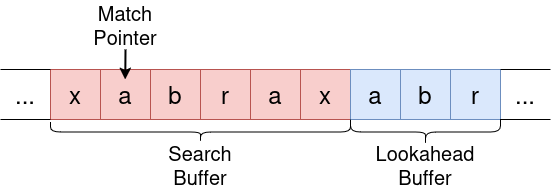
\includegraphics[width=12cm]{figuras/DiagramasTCC-LZ77-template}
  \fonte{Adaptada de \textcite{sayood2012introduction}}
\end{figure}

Este mecanismo permite substituir sequências repetidas por referências a
ocorrências anteriores, resultando em compressões eficazes especialmente para
dados com alta redundância.

% Aqui
\subsection{Exemplo de Codificação com LZ77}\label{sec:LZ77_exemplo}

Nesta seção será demonstrado um exemplo detalhado do funcionamento da janela
deslizante e da representação do token $\langle p, \ell, x \rangle$ utilizados
pelo algoritmo LZ77. 

A sequência a ser codificada é \texttt{"cabracadabrarrarrad"}. Para este exemplo, a janela deslizante possui
um tamanho total fixo de 13 caracteres, com o \textit{lookahead buffer}
definido em 6 caracteres. O estado inicial da janela pode ser visto na
Figura~\ref{fig:Estado_0_LZ77}.

\begin{figure}[htp]
  \centering
  \caption{Estado inicial da janela deslizante no algoritmo LZ77}
  \label{fig:Estado_0_LZ77}
  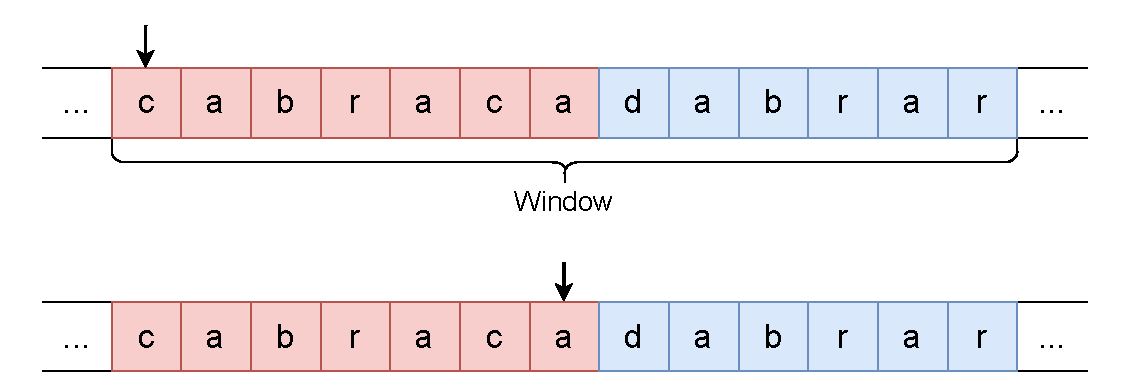
\includegraphics[width=15cm]{figuras/DiagramasTCC-LZ77-Estado-0.pdf}
  \fonte{Adaptada de \textcite{sayood2012introduction}}
\end{figure}

Inicialmente, busca-se no \textit{search buffer} , da esquerda para direita, algum caractere ou sequência
que coincida com o início do \textit{lookahead buffer}. Neste momento,
deseja-se codificar o primeiro caractere do \textit{lookahead buffer}, que é
\texttt{"d"}. Ao observar o \textit{search buffer}, verifica-se que não há
nenhuma correspondência prévia para este caractere. Portanto, o algoritmo gera
o token $\langle 6, 0, \texttt{d} \rangle$, indicando que não houve
correspondência, apesar de o pointer ser 6, o comprimento da sequência
 é 0, assim não fazendo a diferença na codificação, pois não existe cópia sendo feita.

Após esta codificação inicial, a janela deslizante avança uma posição, o que
altera o conteúdo tanto do \textit{search buffer} quanto do \textit{lookahead
  buffer}, conforme mostrado na Figura~\ref{fig:Estado_1_LZ77}.

\begin{figure}[htp]
  \centering
  \caption{Estado da janela após primeira codificação no algoritmo LZ77}
  \label{fig:Estado_1_LZ77}
  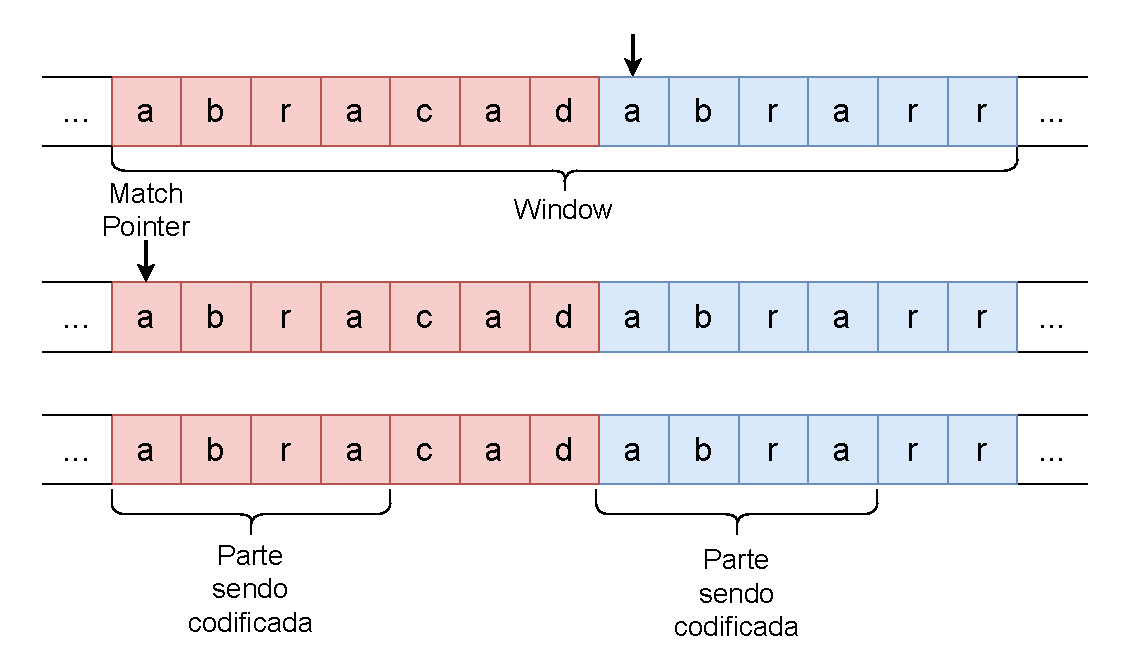
\includegraphics[width=15cm]{figuras/DiagramasTCC-LZ77-Estado-1.pdf}
  \fonte{Adaptada de \textcite{sayood2012introduction}}
\end{figure}

Nesse novo estado, procura-se novamente uma correspondência no \textit{search
  buffer} para a sequência do \textit{lookahead buffer}, que agora começa com
\texttt{"a"}. Observando o \textit{search buffer}, é possível encontrar
múltiplas ocorrências isoladas do caractere \texttt{"a"}, próximo a esquerda. Notavelmente, existe uma
sequência completa \texttt{"abra"} previamente codificada, iniciando a
0~caracteres de distância da posição atual da janela. Essa correspondência
possui comprimento 4~caracteres.

Dessa forma, o algoritmo codifica a sequência encontrada como o token $\langle
  0, 4, \texttt{r} \rangle$, onde $0$ indica a distância até o início da
correspondência no \textit{search buffer}, $4$ indica o comprimento da
correspondência encontrada (\texttt{"abra"}), e \texttt{"r"} é o caractere
seguinte imediatamente após essa sequência, ainda não codificado. Após isso, a
janela avança em 5~posições (4~caracteres da sequência codificada mais
1~caractere literal).

Para realizar o processo inverso, ou seja, decodificar o token recebido
$\langle 0, 4, \texttt{r} \rangle$, o decodificador utiliza o mesmo princípio
do algoritmo LZ77, porém no sentido inverso.

Inicialmente, ele utiliza o offset ($o$) para retornar exatamente 0 posições na
sequência já decodificada até o momento. A partir dessa posição inicial
encontrada, copia-se uma sequência de comprimento 4 (valor $l$), obtendo o
trecho \texttt{"abra"}. Em seguida, adiciona-se ao final desta sequência
copiada o caractere literal adicional ($c$), que neste exemplo é \texttt{"r"}.

Esse processo é ilustrado passo a passo na Figura~\ref{fig:Estado_deconding}.
Inicialmente, há o estado parcial da decodificação com o \textit{buffer} já
reconstruído. Em seguida, avança-se caractere a caractere, copiando-se do
\textit{buffer} reconstruído e adicionando o caractere literal no final. O
resultado final após a decodificação deste token será \texttt{"abrar"}.

Vale destacar que o decodificador reconstrói o buffer de busca dinamicamente,
conforme recebe e processa novos tokens, permitindo a reconstrução exata dos
dados originais sem perda alguma.

% Até Aqui

\begin{figure}[htp]
  \centering
  \caption{Decodificação do exemplo $\langle 7, 4, \texttt{r} \rangle$ }
  \label{fig:Estado_deconding}
  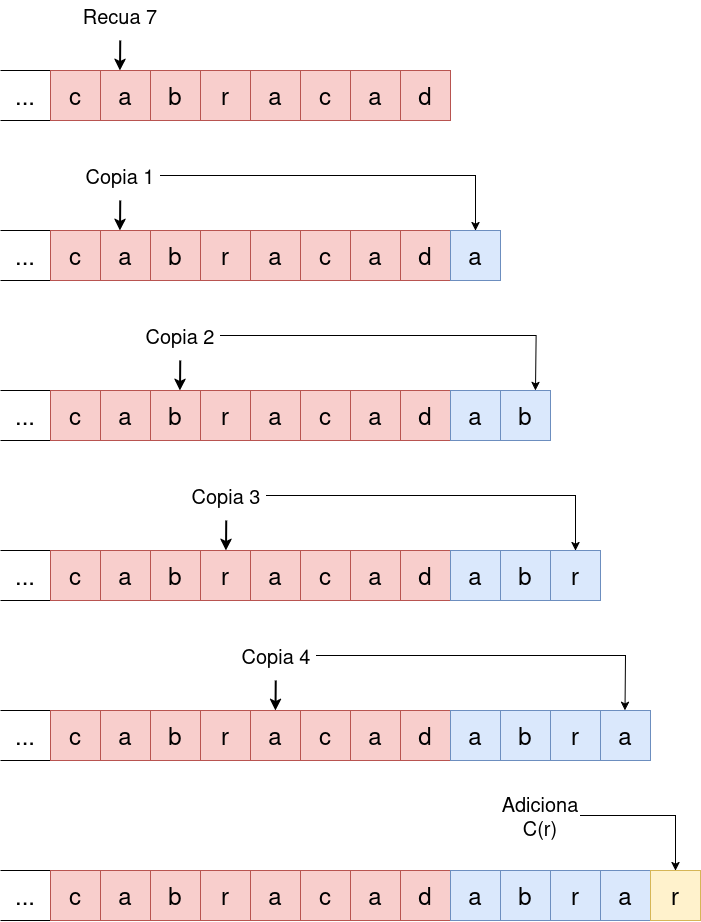
\includegraphics[width=12cm]{figuras/DiagramasTCC-LZ77-Decoding}
  \fonte{Adaptada de \textcite{sayood2012introduction}}
\end{figure}

Utilizando o exemplo anterior do token $\langle 7, 4, \texttt{r} \rangle$, onde
a janela total possui 13 caracteres, temos a seguinte definição dos campos em
bits:
\begin{itemize}
  \item O deslocamento ($p$) pode variar de 0 a 6, portanto requer $3$~bits;
  \item  O comprimento ($\ell$) pode variar de 0 a 7, logo exige também $3$~bits;
  \item O caractere literal ($c$) é codificado em ASCII, utilizando $8$~bits
        ($1$~byte).
\end{itemize}
Dado que na implementação adotada os tamanhos em bits para cada campo do token são
\[
  \underbrace{3}_{\substack{\text{bits para}\\\text{pointer }($p$)}} +
  \underbrace{3}_{\substack{\text{bits para}\\\text{length }(\ell)}} +
  \underbrace{8}_{\substack{\text{bits para}\\\text{character }(x)}}
  = 14\;\text{bits},
\]
temos um formato de código de comprimento fixo, no qual cada token $\langle p,
  \ell, x\rangle$ ocupará exatamente 14 bits. Em outras palavras, após definido o
tamanho da janela (\textit{pointer}) e do \textit{lookahead buffer}
(\textit{length}), bem como o padrão de 8 bits para o caractere literal, toda e
qualquer codificação produzida por esse esquema terá comprimento contínuo de 14
bits por símbolo codificado \cite{nelson2008data}.

Realizando a codificação especificamente para o exemplo dado ($\langle 0, 4,
  \texttt{r} \rangle$), obtêm-se:
\begin{itemize}
  \item O valor do \textit{offset} $o = 0$, em $3$ bits é $000_{(2)}$.
  \item O comprimento $l = 4$, em $3$ bits é $100_{(2)}$.
  \item O caractere $r$, em ASCII binário ($8$ bits), é $01110010_{(2)}$.
\end{itemize}
Portanto, a representação completa do token em bits será:
$$
  000 \;|\; 100 \;|\; 01110010
$$
Resultando na sequência binária final: $00010001110010_{(2)}$.

Esse processo ilustra o funcionamento fundamental do algoritmo LZ77, mostrando
como ele explora redundâncias por meio de correspondências encontradas em
trechos já codificados, reduzindo o volume de dados transmitidos ou
armazenados.

% Revisões Aqui
\newpage
\section{Biblioteca Komm}
A \textit{Komm} é uma biblioteca em \textit{Python} para sistemas de
comunicação desenvolvida pelo professor Roberto Nobrega. Trata-se de um projeto
\textit{open-source} para \textit{Python 3} que fornece ferramentas para
análise e simulação de sistemas de comunicação analógicos e digitais.

Este projeto foi inspirado em diversas outras bibliotecas para sistemas de
comunicação, como \textit{MATLAB\textsuperscript{\textregistered}
  Communications System Toolbox\texttrademark}, \textit{GNU Radio},
\textit{CommPy} e \textit{SageMath}.

Além disso, a biblioteca já disponibiliza diversas codificações implementadas,
abrangendo diferentes técnicas de \textit{source coding} e \textit{lossless
  coding}, incluindo:
\begin{itemize}
  \item {Shannon Code}
  \item {Fano Code}
  \item {Huffman Code}
  \item {Tunstal lCode}
  \item {LZ78}
  \item {LZW}
\end{itemize}

\chapter{Desenvolvimento}\label{cap:desenvolvimento}

Este capítulo descreve o desenvolvimento dos módulos LZ77 na biblioteca \textit{Komm}. A implementação foi realizada em
Python, linguagem-base do projeto.

\section{Módulo LZ77}

Esta seção documenta a implementação do algoritmo \textit{Lempel–Ziv 77} (LZ77)
na \textit{Komm}, cobrindo decisões de projeto, integração e validação. A
biblioteca já inclui diversos esquemas de compressão sem perdas (Huffman,
Tunstall, LZ78 e LZW), e a contribuição aqui foi a implementação completa do
LZ77 com foco tanto prático quanto didático.

\subsection{Objetivos e escopo}

Os objetivos deste módulo foram:
\begin{itemize}
    \item implementar as rotinas de codificação (\texttt{encode}) e decodificação
          (\texttt{decode}) gerando \textbf{tokens} no formato \((p,\ell,x)\);
    \item integrar a classe ao padrão já utilizado, documentação e testes da \textit{Komm};
    \item disponibilizar uma \textbf{pipeline modular} para fins educacionais,
          viabilizando a inspeção de resultados intermediários e a comparação com
          exemplos da literatura (que, em geral, não mostram a saída em base binária).
\end{itemize}

\subsection{Janela deslizante e notação}\label{subsec:janela-notacao}

Adotamos a notação usadas nas bibliografias que foram utilizadas para o estudo do algoritmo LZ77:
\[
    W = S + L,
\]
onde \(S\) é o tamanho do \emph{search buffer}, \(L\) é o tamanho do
\emph{lookahead buffer} e \(W\) é o tamanho total da janela. Denotamos por \(
|\mathcal{X}| \) a cardinalidade do alfabeto de \textbf{entrada} e por \(
|\mathcal{Y}| \) a cardinalidade do alfabeto de \textbf{saída}.

Cada token tem o formato
\[
    (p,\ell,x),
\]
em que \(p\) é o \textit{pointer} (deslocamento no \emph{search buffer}),
\(\ell\) é o comprimento da ocorrência e \(x\in \mathcal{X}\) é o símbolo
literal subsequente.

\paragraph*{Origem do ponteiro.}
Neste trabalho, seguindo o artigo original do LZ77, \(p\) é medido a partir do \textbf{início} do \emph{search buffer}. \emph{Observação}: algumas implementações didáticas medem a partir do \textbf{fim} do \emph{search buffer}; ambas convenções aparecem na literatura. Mantemos a primeira e documentamos a diferença quando necessário.

\subsection{Arquitetura e estrutura da implementação}

A classe \texttt{LempelZiv77Code} concentra a lógica do algoritmo e expõe a classe da seguinte maneira:
\begin{lstlisting}[language=Python, caption={Estrutura simplificada da classe LZ77}]
@dataclass
class LempelZiv77Code:
    source_cardinality: int      # |X|
    target_cardinality: int      # |Y|
    window_size: int             # W
    lookahead_size: int          # L (logo S = W - L)

    def encode(self, data): ...
    def decode(self, encoded): ...
\end{lstlisting}

Exemplo de uso:
\begin{lstlisting}[language=Python, caption={Uso típico do LZ77 na \textit{Komm}}]
lz77 = LempelZiv77Code(
    source_cardinality=256,     # |X|
    target_cardinality=2,       # |Y| (binário)
    window_size=32768,          # W
    lookahead_size=258          # L (então S = 32510)
)
encoded = lz77.encode(b"... dados ...")
decoded = lz77.decode(encoded)
assert decoded == b"... dados ..."
\end{lstlisting}


Com intuito pedagógico, a pipeline foi dividida em \textbf{quatro} módulos
internos — dois para \texttt{encode} e dois para \texttt{decode}:
\begin{enumerate}
    \item \textbf{Codificação}
          \begin{itemize}
              \item \texttt{source\_to\_tokens}: identifica os tokens \((p,\ell,x)\) sobre a janela \(W=S+L\);
              \item \texttt{tokens\_to\_target}: mapeia os tokens para o fluxo no alfabeto de saída \(\mathcal{Y}\).
          \end{itemize}
    \item \textbf{Decodificação}
          \begin{itemize}
              \item \texttt{target\_to\_tokens}: reconstrói os tokens a partir do fluxo em \(\mathcal{Y}\);
              \item \texttt{tokens\_to\_source}: recompõe a sequência original em \(\mathcal{X}\).
          \end{itemize}
\end{enumerate}

Essa organização favorece: (i) clareza didática; (ii) comparação direta com
esquemas de manuais/artigos; e (iii) inspeção de saídas intermediárias
(inclusive em binário), recurso raramente mostrado na literatura.

\subsection{Larguras de campos na saída}\label{subsec:larguras}

Seja a saída codificada em base \( |\mathcal{Y}| \). As larguras (em símbolos
do alfabeto de saída) dos campos do token são:
\[
    w_p = \big\lceil \log_{|\mathcal{Y}|} S \big\rceil,\qquad
    w_\ell = \big\lceil \log_{|\mathcal{Y}|} L \big\rceil,\qquad
    w_x = \big\lceil \log_{|\mathcal{Y}|} |\mathcal{X}| \big\rceil,
\]
e o custo total por token é
\[
    n \;=\; w_p + w_\ell + w_x.
\]

\subsection{Testes e validação}\label{subsec:testes}

Os testes unitários (\texttt{test\_lz77.py}) cobrem:
\begin{itemize}
    \item cadeias com alta redundância e com sobreposição;
    \item exemplos reproduzidos da literatura.
\end{itemize}
A validação principal usa \textit{round trip} (\(\texttt{decode}(\texttt{encode}(x)) = x\)) e compara tokens/fluxos intermediários com os parâmetros \((W,S,L)\) e larguras \((w_p,w_\ell,w_x)\).



\chapter{Resultados}\label{cap:Resultados}
A partir dos algoritmos implementados na biblioteca \textit{Komm}, foram realizados testes de compressão e descompressão com diferentes conjuntos de dados. Este capítulo apresenta os resultados obtidos, incluindo análises de desempenho e comparações com outras bibliotecas populares encontradas no github.

Para esta secção, foram utilizados 2 tipos de arquivos: arquivos de texto e arquivos de imagem. Os arquivos de texto foram escolhidos por serem comuns em aplicações de compressão, enquanto os arquivos de imagem foram selecionados para avaliar o desempenho.
Os arquivos utilizados foram:
\begin{itemize}
    \item \textbf{Arquivos de Texto:} Alice’s Adventures in Wonderland
    \item \textbf{Arquivos de Imagem:} Imagens no formato bitmap (BMP)
\end{itemize}
O arquivo de texto utilizado foi o livro "Alice’s Adventures in Wonderland", disponível no projeto Gutenberg\footnote{https://www.gutenberg.org/ebooks/11}. Este arquivo é representativo de textos literários e possui uma variedade de caracteres e padrões que são úteis para testar algoritmos de compressão.
As imagens no formatos .bmp podem ser vizuliadas na Figura \ref{fig:smiley} e \ref{fig:snail}.

\begin{figure}[h]
	\centering
	\caption{Imagem no formato bitmap (BMP) de um smiley}
	\label{fig:smiley}
	
\includegraphics[width=5cm]{figuras/smiley-large.png}
    \fonte{https://cse1.net/recaps/graphics}
\end{figure}

\begin{figure}[h]
	\centering
	\caption{Imagem no formato bitmap (BMP) de um caracol}
	\label{fig:snail}
	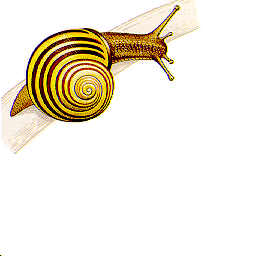
\includegraphics[width=5cm]{figuras/snail.png}
    \fonte{https://people.math.sc.edu/Burkardt/data/bmp/bmp.html}
\end{figure}

\pagebreak
\section{Métricas de Avaliação}
Para avaliar o desempenho dos algoritmos de compressão implementados na biblioteca \textit{Komm}, foram utilizadas as seguintes métricas:
\begin{itemize}
    \item \textbf{Taxa de Compressão:} A taxa de compressão é definida como a razão entre o tamanho do arquivo original e o tamanho do arquivo comprimido. Uma taxa de compressão maior indica uma melhor eficiência do algoritmo.
    \item \textbf{Tempo de Compressão e Descompressão:} O tempo gasto para comprimir e descomprimir os arquivos também foi medido. Tempos menores indicam um desempenho melhor do algoritmo.
    \item \textbf{Utilização de Memória:} A quantidade de memória utilizada durante o processo de compressão e descompressão foi monitorada para avaliar a eficiência do algoritmo em termos de recursos computacionais.
    \item \textbf{Integridade dos arquivos: } Após a descompressão, os arquivos foram comparados com os arquivos originais para garantir que não houve perda de dados durante o processo de compressão e descompressão.
\end{itemize}

\section{Resultados Obtidos}




% Imprimir Referências
\printbibliography[title={Referências}]%

%-----------------------------------------------%
% Apêndices
%-----------------------------------------------%
\begin{apendicesenv}


\chapter{Meu primeiro apêndice}

Texto ou documento, elaborado pelo autor, a fim de complementar sua argumentação, sem prejuízo da unidade nuclear do trabalho. Os apêndices são identificados por letras maiúsculas ordenadas alfabeticamente, travessão e pelo respectivo título. 

\end{apendicesenv}

% Anexos
%-----------------------------------------------%
% Anexos
%-----------------------------------------------%
\begin{anexosenv}


\chapter{Meu primeiro assunto de anexo}

Texto ou documento não elaborado pelo autor, que serve de fundamentação, comprovação e ilustração. Os anexos são identificados por letras maiúsculas ordenadas alfabeticamente, travessões e pelos respectivos títulos. 

\chapter{Segundo assunto que pesquisei}
\lipsum[1-3]

\end{anexosenv}


\end{document}